In this chapter it is explained how the tool has been developed. The first section is describing the coding languages used and the plugins used to create the tool. The following sections are describing the necessary steps to build the tool. These steps can be seen in figure \ref{DevelopmentSteps}.

\begin{figure} [H]
	\centering
	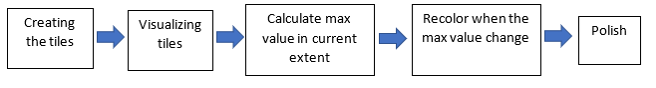
\includegraphics[width=.8\textwidth]{Pictures/DevelopmentSteps}
	\caption{An overview of the code}
	\label{DevelopmentSteps}
\end{figure}

First it is necessary to divide the raster into tiles to be able to limit the loaded data to the current extent. How this is done is explained in section x. Section x describes how the tiles have been visualized. To be able to color the tiles based on the current values it is required to know what the current values are. In section x it is explained how this information is calculated. The raster layer is then rerendered with these values as described in section x. Lastly some measurements were taken to ensure a more user-friendly experience. These additions are described in section x. 

\chapter{Coding languages and plugins}
For this project, the coding language Python was used to create the tiles, while visualization of the tiles was done in a webgis build with the languages HTML, CSS and Javascript. This webgis have been tested on a local caddy server for reasons explained in section x

\section{Languages}
\subsection*{Python}
Python is programming language with a simple syntax, which functions across multiple different platforms. This simple syntax means that Python can achieve the same as some other coding languages in fewer lines. $https://www.w3schools.com/python/python_intro.asp$
Python was used in this project because of the gdal library expanded further upon in section x
This project has been using version 3.6 of Python. 
\subsection*{HTML}
HTML is short for Hyper Text Markup Language. It is the language used for defining and structuring a web page’s content.
https://www.w3schools.com/js/default.asp
\subsection*{CSS}
CSS is an abbreviation for Cascading Style Sheets. This language defines how the HTML will be displayed.
\subsection*{Javascript}
How a webpage behaves is defined by the language Javascript.  This is what makes the web page interactive. 
\citep{CPL}

\section{Libraries}
To transform the raster data into smaller tiles the python library Gdal is used. 
\subsection*{Gdal}
GDAL is library for translating between multiple different geospatial data formats. https://gdal.org/ 

Included in this library is the gdal2tiles program, which can divide raster files into smaller tiles. 
At the time of using this program it was only able to generate tiles structured after the TMS standard. The function to follow the XYZ structure was added the 3th of May 2020 https://gdal.org/programs/gdal2tiles.html
%https://gdal.org/download.html#current-releases 
The script rendering the tiles in the map was based on the XYZ structure. This meant that the rows of tiles were ordered incorrectly when the generated tiles were imported. Therefore, the official version of gdal2tiles was replaced by a version made by a github user named commenthol. This version is modified to allow the creation of tiles following the XYZ structure. 
https://github.com/commenthol/gdal2tiles-leaflet
Both the official version and the modified version have their output format as mbtiles with a bit depth of 8 bit. To be usable for this project a bit depth of at least 32 bit is needed, as mentioned in section x. The workaround for this issue will be explained in section x. 
\subsection*{Openlayers}
The map in which the tiles are being showed are created in Openlayers, which is an open source JavaScript library for creating dynamic maps for web pages. 
https://openlayers.org/
Openlayers was chosen because the tool presented in related work was built in Openlayers. Therefore, using Openlayers would enable expanding upon this existing tool instead of starting from scratch. 

\subsection*{olGeoTiff}
olGeoTiff is a Javascript class for visualising geotiff tiles in Openlayers, utilising the libraries geotiff.js and Plotty. The visualized tiles are being processing in the client instead of on a server. It was used in the map presented in section x. 
The class is a modified version of Openlayers WMTS layer, where the internal tile loading function has been changed. The regular function would request precolored tiles and then add them to the map. The tiles requested by the modified version are not precolored and need to be processed before getting added to the map. A simplified illustration of this processing is illustrated in figure x. This simplified figure is enough to explain the mechanics of the class but does not detail the callback function structure. Aside from being used for error handling callbacks are also necessary to ensure that Openlayers do not try to add the tiles to the map, before they have been processed. More detailed figures can be found in Bernhard Baumrocks thesis.

\begin{figure} [H]
	\centering
	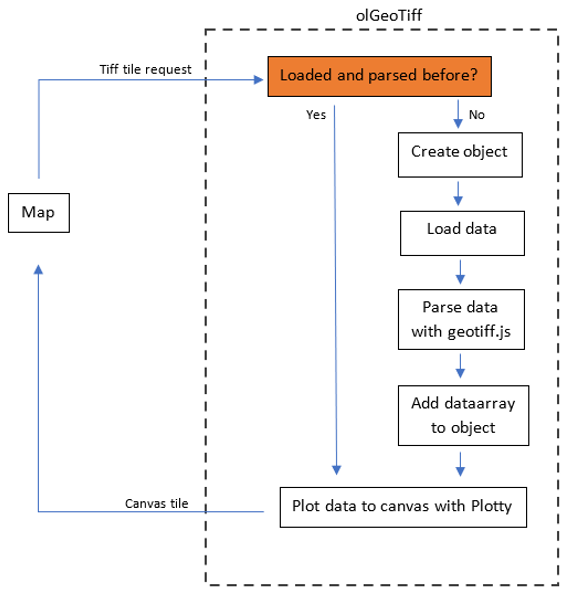
\includegraphics[width=.8\textwidth]{Pictures/olGeoTiffSimplified}
	\caption{A simplified illustration of how olGEoTiff functions}
	\label{olGeoTiffSimplified}
\end{figure}

To ensure that tiles are only being downloaded once an object keeps track of all the downloaded data. The object is organized by the tiles’ url. 
Whenever tiles are being requested the object will always be checked to see if it already contains the url. If it does not the object will be updated to include the requested tile. The tile will then be loaded before being processed. 
The processing is done with the TIFF parser geotiff.js 
https://geotiffjs.github.io/
and Plotty, which is a library for creating images from data arrays.
https://github.com/santilland/plotty
. The loaded tiles first get parsed with geotiff.js and added to the object before Plotty get used to render tiles in the designated colors. Then the tiles get added to the map.
\citep{BThesis}
https://web.archive.org/web/20191031034339/https://eox.at/2018/01/visualizing-geotiff-tiles-with-openlayers/
The olGeoTiff also have a redraw function, which when triggered will redraw the tile layer based on the current designated colors. This was for instance used in Bernnard Baumrocks map, whenever the color sliders were changed. 

%\section{Testserver}
%Not finished
%The solution was being tested in Google Chrome initially using a python-based http server. This was later replaced with a Caddy server to improve performance. 
% 
%Caddy
%http’s limits to 6 connections 
%fig text: Blue: DomContentLoaded Red: Load